\chapter{Integration}
\section{Methods}
The integration of the system was performed by individually implementing each sub-section
and ensuring that the sub-section's outputs are compatible with adjacent sub-section inputs.

With this methodology in mind, the system was integrated in the order of outputs to inputs.
This is so that with the edition of each new sub-section, the system response to the new sub-section can be verified.

First, the lighting controller was implemented, as shown in the Lighting Controller chapter.
Then, software for the off-body PC was written that could communicate with the lighting controller,
and control the prototyping fixture based on a prerecorded dataset.
The dataset was that of an electrocardiogram sampled at 360 Hz.
The lights were controlled by pulsing their intensity at the peaks of the electrocardiogram.
Then, the software was modified so that the data being processed could be received as a continuous stream, instead of a fixed dataset.

Communication between the on-body device and the off-body PC has already been documented in the On-Body Device chapter.
This communication was expanded upon by receiving the data into the same continuous stream that had already been established with the dataset,
thus allowing the on-body device to control the prototyping fixture through peaks in the transmitted data.

The on-body device needs to collect different types of data with varying sample and transmission rates.
Much like implementing the prototyping fixture for the lighting controller where the end of each DMX frame needed to be marked,
the varying data sizes were implemented using special characters to mark the end of data transmission using base64.
Additionally, packet headers were created to specify the different kinds of data that are being sent
(implementation was prior to the board power distribution issues).


\section{Results}
The off-body PC has a fixed length first-in-first-out buffer that can be filled with either testing data or streamed data from the on-body device.
The received data can control the prototyping fixture, with various methods of control through data processing.
Beat detection was implemented on the testing dataset,
allowing the prototyping fixture to increase intensity at each peak of the input data.

\begin{figure}[!ht]
  \caption{Fixed length FIFO data buffer with testing dataset}\label{fig:matlab_packet_test2}
  \centering
  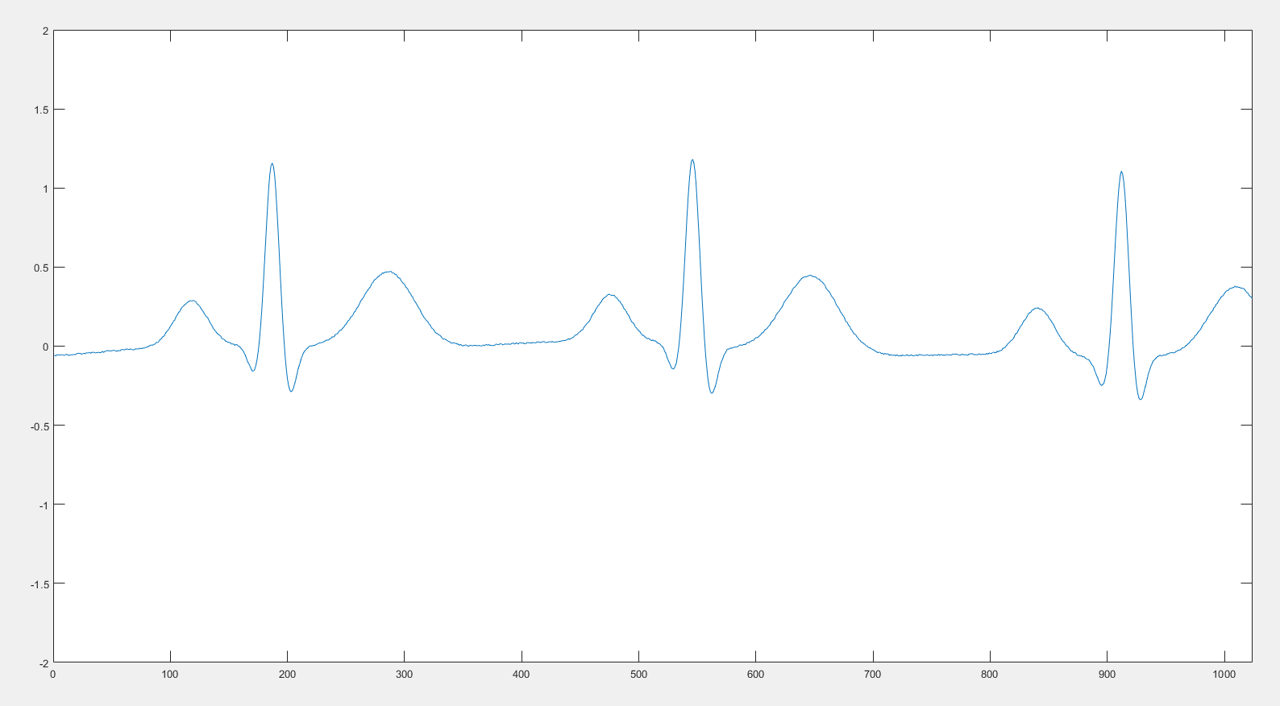
\includegraphics[width=1\columnwidth]{chapters/development/MATLAB/FULL_FILLED}
\end{figure}

The implementation of varying data sizes and the inclusion of packet headers allows data to be effectively transmitted and received.
An unintended benefit of this is that a debug packet header can be specified, and since the data can be variable length,
a fully functional `printf' function on the PIC32 can be used to send arbitrary debugging messages to the off-body PC.

As was presented in the On-Body Device chapter, the PIC32 and ESP32 are able to communicate with the off-body PC at a speed of 1.45 kbits/s.
At a sampling rate of 50 Hz~\cite{Ajdaraga:2017}, the bandwidth is high enough to send 29 bits.
For instance, you could send 8-bits of header information and 16-bits of electrocardiogram data, while maintaining sampling and transmitting at 50 Hz.


\section{Discussion}
To reduce the amount of hardware that is required to be worn by the performer,
the bulk of the processing is to be done on an off-body PC.
This PC communicates wirelessly with the on-body device,
receiving sensor data from the various biosignals that the device is measuring.
The PC then must process the data and coordinate the music and lighting generation.

% TODO: WOULD BE GOOD TO HAVE A DECISION MATRIX HERE
MATLAB was used as the off-body PC language for processing because of ease of use, versatility,
and previous usage on this project.

Since MATLAB functions operate on arrays and matrices,
the desired behaviour of our program is to store a length of data and process it all together,
rather than try to process each sample individually as it arrives.
To keep the system responsive, the buffer is kept at a fixed length,
so that over time the processing does not incrementally take longer due to the increase in data to process.
To achieve this, the number of samples added to the front of the buffer need to be removed from the rear of the buffer each time a new sample is received.
An `offline' version of this program can be made without the need for full system integration using previously saved sampled data.
Since this data is the same as what we will be eventually expecting to see,
The processing code that we write for this test data will also function similarly on the real data.

For testing, an electrocardiogram (ECG) data-set from a previous iteration of the project was used.
The load command will load a number of different ECG data-sets with that all have different beats per minute (BPM),
and the desired ECG signal for testing can be selected by changing the the assignment of the ECG variable.
For example, to load a 60 BPM ECG signal, the assignment could be changed to ECG = ecgdata360Hz\_hrmean60.
The specific data-sets that are available can be seen in the workspace tab of MATLAB once the load command has been executed.
Additionally, a loop rate is calculated to simulate the sensor sampling rate.
Since the testing data-set sample rate is known, it can be easily calculated from that.

Once the data-set has been imported, the program can loop through and generate example packets for testing.

The first thing that is done is the constants and variables definitions.
In this context, packet refers to the small subset of the ECG signal that is going to be added to the larger fixed length array.
That fixed length array is labelled `data' in this example.

The packet index is the data position from the ECG data-set where data will be sampled from.
Packet length determines how many samples at a time are shifted in and out of the data array,
this is to simulate the device transmitting multiple samples at a time.

When the packet index reaches the end of the ECG data-set, the index resets back to the beginning.
This is so the test program can run continuously, regardless of how big the test data-set actually is.
When the index resets, there is a break in continuity of the signal. However, this is a known issue and can be easily detected and ignored.

% TODO: FIGURE SHOWING DATA ENTERING AND EXITING FIXED LENGTH ARRAY
The fixed data array can then be updated by first shifting the current data to the left, disposing of packet length worth of data at the beginning.
Then, the same amount of data, from the packet, can be appended to the end of the array.
Plots of this data are shown in~\autoref{fig:matlab_packet_test1} and\autoref{fig:matlab_packet_test2}.

With this setup, the off-body PC is ready to process an incoming signal as a fixed sized array of data.

% TODO: WOULD BE GOOD TO HAVE SOME RESULT FROM THIS IN SOME CAPACITY
This code calculates the BPM of the signal by measuring the gaps between the peaks of the ECG QRS signals.
It can be verified by comparing the measured BPM value with the given value from the data-set.
When the system is integrated, as long as the data length matches and the sensor data is accurate,
this same code will produce similar results.

With all the block of the system functional,
the first step of system integration is to establish communication between the off-body PC and on-body device.

On the on-body device, the ESP32 acts as the wireless bridge.
As this device requires a connection to WiFi for OTA updates, the wireless protocol that was chosen to be implemented was TCP/IP.
This is because the device already has a TCP/IP requirement and the only other choice for wireless communication was Bluetooth, which does not have the range or speed that TCP/IP has.

In order to get these devices to communicate, inbound and outbound rules need to be defined in the off-body PC firewall.
This is to allow connections on the specified port, since most PC ports are typically closed for security reasons.
The port settings can be seen in~\autoref{fig:firewall}.

\begin{figure}[!ht]
  \caption{TCP/IP firewall port settings}\label{fig:firewall}
  \centering
  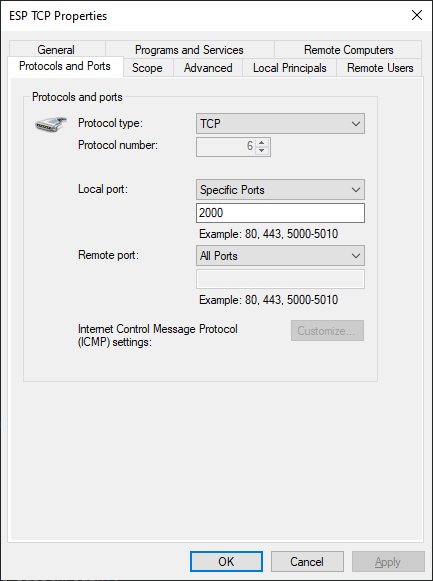
\includegraphics[width=1\columnwidth/2]{chapters/development/FIREWALL}
\end{figure}

With data being sent between the ESP32 and the off-body PC, the next device to connect is the PIC32 to the off-body PC.
Since the SPI communication between the PIC and the ESP has already been established,
the process buffer task can be updated to pass-through the received data to the off-body PC.

Sending individual bytes between devices is now possible.
Currently, this only works as long as the value fits into a predetermined number of bytes.
Additionally, once the system is running with non-known values, there is no easy way to keep the data synchronized.
For instance, if a byte of data was lost, the received data would be in the incorrect place
and there would be no way of knowing.
This could be solved by sending a known byte sequence at the beginning of transmission.
However, there would be no differentiation between that byte sequence and any arbitrary data that may be being sent.
Another approach is to limit the character set so that specific byte values can correspond to `special' characters.
For example, the decimal value of 10, which corresponds to the newline character, could be used to mark the end of transmission.
That way, even if the transmitter and receiver become out of sync, the system has a way of recovering.
There are a number of character sets that have already been developed.
For this project, base64 was implemented due to its lower overhead when compared to ASCII, its human readability to aid debugging, and its good documentation.

This code takes the inputted data and limits it to only use characters from the encoding table.
After the data has been encoded, it is sent to the ESP32 for writing to the off-body PC.

With this implemented, data that is sent to the off-body PC is consistently received correctly and the devices do not get out of sync.
This encoding function allows for arbitrary data to be sent between the PIC32 and the off-body PC.
One major benefit of this is that it allows custom wrapping of a printf function, along with the previously implemented packet writing function,
to give the user a custom debugging function that allows any number or string to be formatted and sent to the off-body PC.

Then, the program can be debugged using printf.
This allows the device to continue running while providing feedback, rather than needing to be put into debugging mode and stepped through manually.
The primary benefit of this is that it provides information without disrupting timings such as the use of breakpoints does, also this allows debugging in callback functions,
which the debugger conventionally cannot step into.

The final part of the project is the testing and validation.
While all of the independent parts of the system had been tested in a vacuum,
unfortunately when the system was fully operational, the device failed due to power supply issues.
The issues are related to what was seen earlier with the ESP32 power issues.
As more devices came online, the current draw across on-body device's power plane increased, which subsequently increased the voltage drop.
Eventually, this voltage drop became too large and the devices started to lose power.
Thus, the testing and validation of the system remains unfinished, as the device was no longer responsive at the point when testing began.
